% =============================================================================
\section{Binding Modules}
\label{sec:modules}
% =============================================================================
We describe the bindings generated by our system for various \cgal{} packages and exemplify the use of the generated bindings.
%
When developing code in Python that uses the bindings, the statement that imports the binding library, that is,
\begin{lstlisting}[style=pythonStyle]
>>> import CGALPY
\end{lstlisting}
must precede any statement that use the binding. This statement is omitted in all examples hereafter.
%
For lack of space, we defer description of the kernel modules to Appendix~\ref{sec:kernelModules}.

% -----------------------------------------------------------------------------
\subsection{2D Arrangement Bindings}
\label{ssec:modules:aos2}
% -----------------------------------------------------------------------------
Given a surface $S$ in \Rthree{} and a set $\calC$ of curves embedded in this surface, the curves subdivide $S$ into cells of dimension~$0$ (vertices),~$1$ (edges), and~$2$ (faces). This subdivision is the arrangement $\calA(\calC)$ induced by $\calC$ on $S$~\cite{fhw-caass-12}. Arrangements embedded in curved surfaces in \Rthree{} are generalizations of arrangements embedded in the plane. The \iiDArrangementsPackage{} package~\cite{cgal:wfzh-a2-21a} can be used to construct, maintain, alter, and display 2D arrangements embedded in ruled curved surfaces. It also supports queries on such arrangements, such as point location, and other operations. One of the main components of the \iiDArrangementsPackage{} package is the \cppLstinline{Arrangement\_2<Traits, Dcel>} class template. An instance of this template is used to represent an arrangement embedded in the plane.  Table~\ref{tab:aos} lists the \cmake{} flags associated with the \iiDArrangementsPackage{} module.  Currently, only instances of the \cppLstinline{Arrangement\_2<Traits,Dcel>} class template are supported. A description of the two template parameters of this class template follows.

%%%%%%%% Arrangement Module Flags
\begin{table}[!htp]
 \caption{\iiDArrangementsPackage{} module flags. \textbf{Def.} stands for \textbf{Default Value}.}
  \centering\begin{tikzpicture}
  \matrix (first) [tableModuleFlags,
    row 3/.style={nodes={minimum height=2.8em}},
    row 4/.style={nodes={minimum height=2.8em}},
    row 5/.style={nodes={minimum height=2.8em}},
    row 6/.style={nodes={minimum height=5.4em}},
    column 1/.style={nodes={text width=16em}},
    column 2/.style={nodes={text width=4em}},
    column 3/.style={nodes={text width=6.3em}},
    column 4/.style={nodes={text width=11.4em}}
  ] {
    Name & Type & Default & Description\\
    \cmakeLstinline{AOS2\_GEOMETRY\_TRAITS\_NAME} & \cmakeLstinline{String} &       \myLstinline{segment} & The basic geometry traits\\
    \myLstinline{AOS2_EXTEND_VERTEX} & \cmakeLstinline{Boolean} & \myLstinline{false} & Determines whether to extend the vertex type\\
    \myLstinline{AOS2_EXTEND_HALFEDGE} & \cmakeLstinline{Boolean} & \myLstinline{false} & Determines whether to extend the halfedge type\\
    \myLstinline{AOS2_EXTEND_FACE} & \cmakeLstinline{Boolean} & \myLstinline{false} & Determines whether to extend the face type\\
    \myLstinline{AOS2\_POINT\_LOCATION\_BINDINGS} & \cmakeLstinline{Boolean} &       \myLstinline{true} & Determines whether to generate bindings for point location and vertical ray shooting queries\\
  };
 \end{tikzpicture}
 \label{tab:aos}
\end{table}

\begin{itemize}
  \item The Traits template-parameter determines the family of planar curves that induce the arrangement. The parameter should be substituted with a model of the basic arrangement traits concept or one or more concepts that refine the basic concept. A model of the basic traits concept defines the types of x-monotone curves and two-dimensional points and supports basic geometric predicates on them. A rather large directed acyclic graph is required to capture the entire hierarchy of the geometry traits-class concepts. Figure~\ref{fig:atc} depicts two clusters.

  \begin{figure}[!htp]
    \def\name#1{\textsf{\it\footnotesize #1}}
    \tikzset{concept/.style={rectangle split,rectangle split parts=1,draw,
        fill=white,blur shadow,rounded corners,align=center}}
    \captionsetup[subfigure]{justification=centering}
    \centering%
    \subfloat[]{\label{fig:atc:central}
      \begin{forest}
        [\name{AosBasicTraits\_2},for tree={concept,edge={-latex}}
          % forked edges
          [\name{AosXMonotoneTraits\_2}
            [\name{AosTraits\_2}]
          ]
        ]
      \end{forest}}\quad
    \subfloat[]{\label{fig:atc:landmark}
      \begin{forest}
        [\name{AosBasicTraits\_2},name=abt,for tree={concept,edge={-latex}}
          % forked edges
          [\name{AosApproximateTraits\_2}
            [,phantom]
            [\name{AosLandmarkTraits\_2},name=alt,before drawing tree={x=0}]
          ]
          [\name{AosConstructXMonotoneCurveTraits\_2},name=acxmt]
        ]
        \draw[-latex] (acxmt) to (alt);
      \end{forest}}\\
      %
    \subfloat[]{\label{fig:atc:openBoundary}
      \begin{forest}
        [\name{AosBasicTraits\_2},name=abt,before drawing tree={x=0pt},for tree={concept,edge={-latex}}
          % forked edges
          [\name{AosVerticalSideTraits\_2}
            [\name{AosLeftSideTraits\_2}
              [\name{AosOpenLeftTraits\_2},name=olt
                [,phantom]
                [\name{AosOpenBoundaryTraits\_2},name=oyt,before drawing tree={x=0pt}]
              ]
            ]
            [\name{AosRightSideTraits\_2}
              [\name{AosOpenRightTraits\_2},name=ort]
            ]
          ]
          [\name{AosHorizontalSideTraits\_2}
            [name{AosBottomSideTraits\_2}
              [\name{AosOpenBottomTraits\_2},name=obt]
            ]
            [\name{AosTopSideTraits\_2}
              [\name{AosOpenTopTraits\_2},name=ott]
            ]
          ]
        ]
        \draw[-latex] (ort) to (oyt);
        \draw[-latex] (obt) to (oyt);
        \draw[-latex] (ott) to (oyt);
      \end{forest}}\\
      %
    \subfloat[]{\label{fig:atc:sphericalBoundary}
      \begin{forest}
        [\name{AosBasicTraits\_2},name=abt,before drawing tree={x=0pt},for tree={concept,edge={-latex}}
          % forked edges
          [\name{AosVerticalSideTraits\_2}
            [\name{AosLeftSideTraits\_2}
              [,phantom]
              [\name{AosIdentifiedVerticalTraits\_2},name=ivt
                [,phantom]
                [\name{AosSphericalBoundaryTraits\_2},name=sbt,before drawing tree={x=0pt}]
              ]
            ]
            [\name{AosRightSideTraits\_2},name=rst]
          ]
          [\name{AosHorizontalSideTraits\_2}
            [\name{AosBottomSideTraits\_2}
              [\name{AosContractedBottomCurveTraits\_2},name=cbt]
            ]
            [\name{AosTopSideTraits\_2}
              [\name{AosContractedTopCurveTraits\_2},name=ctt]
            ]
          ]
        ]
        \draw[-latex] (cbt) to (sbt);
        \draw[-latex] (ctt) to (sbt);
        \draw[-latex] (rst) to (ivt);
      \end{forest}}
    \caption{%
      (\textbf{\subref{fig:atc:central}})~The central cluster.
      (\textbf{\subref{fig:atc:landmark}})~The landmark cluster.
      (\textbf{\subref{fig:atc:openBoundary}})~The open boundary cluster.
      (\textbf{\subref{fig:atc:sphericalBoundary}})~The spherical boundary cluster.
      }
    \label{fig:atc}
  \end{figure}
  The list of supported traits class templates follows. For each class template we describe the family of curves it handles.
  %
  \begin{compactenum}
  \item \cppLstinline{Arr_non_caching_segment_basic_traits_2<>}---handles
    segments.
  \item \cppLstinline{Arr_segment_traits_2<>}---handles segments,
    where each segment is represented a by its supporting line in
    addition to its two endpoints.
  \item \cppLstinline{Arr_linear_traits_2<>}---handles linear curves,
    i.e., segments, rays, and lines.
  \item \cppLstinline{Arr_polyline_traits_2<>}
  \item \cppLstinline{Arr_polycurve_traits_2<>}
  \item \cppLstinline{Arr_circle_segment_traits_2<>}---handles segments and circular arcs.
  \item \cppLstinline{Arr_conic_traits_2<>}
  \item \cppLstinline{Arr_rational_function_traits_2<>}
  \item \cppLstinline{Arr_Bezier_curve_traits_2<>}---handles B\'ezier curves of arbitrary degrees.
  \item \cppLstinline{Arr_algebraic_segment_traits_2<>}---handles algebraic curves of arbitrary degrees.
  \end{compactenum}

  The \cmake{} flag \myLstinline{AOS2\_GEOMETRY\_TRAITS\_NAME} specifies which geometry traits should be used to define the geometry traits for the generated bindings; see Table~\ref{tab:aos:gt}. Observe that an instance of the \cppLstinline{General_polygon_set_2<>} class template (see Section~\ref{ssec:modules:bso2}) employs a 2D arrangement type. Bindings for instances of \cppLstinline{General_polygon_set_2<>} is enabled as part of the bindings for the \iiDRegularizedBooleanSetOperationsPackage{} package. When bindings for this package is enabled, the traits parameter must be substituted with a traits class that also models the \cppLstinline{GeneralPolygonSetTraits\_2} concept. The appropriate final traits type is automatically defined by the system.
  %
\item The \cppLstinline{Dcel} template-parameter should be substituted with a class that models the \cppLstinline{ArrangementDcel} concept, which is used to represent the topological layout of the arrangement.\footnote{See \url{https://doc.cgal.org/latest/Arrangement_on_surface_2/classArrangementDcel.html}.} This parameter is substituted with an instance of the template \cppLstinline{CGAL::Arr_dcel_base<V, H, F>}, where \cppLstinline{V}, \cppLstinline{H}, and \cppLstinline{F} are models of the concepts\linebreak
\cppLstinline{ArrangementDcelVertex}, \cppLstinline{ArrangementDcelHalfedge}, and \cppLstinline{ArrangementDcelFace}, respectively; by default they are substituted with \cppLstinline{Arr_vertex_base<Traits::Point_2>}, \cppLstinline{Arr_halfedge_base<Traits::X_monotone_curve_2>}, and \cppLstinline{Arr_ face_base}. In many applications it is necessary to extend the types of the DCEL main features. This is governed by three \cmake{} Boolean flags as follows. If any one of the \cmake{} variables \cmakeLstinline{AOS2\_VERTEX\_EXTENDED}, \cmakeLstinline{AOS2\_HALFEDGE\_EXTENDED}, or \cmakeLstinline{AOS2_FACE_EXTENDED} is set to true, the corresponding template parameter, \cppLstinline{V}, \cppLstinline{H}, or \cppLstinline{F}, is substituted with instances of \cppLstinline{Arr_extended_vertex<Vb, VertexData>}, \cppLstinline{Arr_extended_halfedge<Hb, HalfedgeData>}, or \cppLstinline{Arr_extended_face<Fb, FaceData>}, respectively, where \cppLstinline{Vb}, \cppLstinline{Hb}, and \cppLstinline{Fb} are the basic types above.
%
  It is impossible to define a custom C++ type from Python code. Therefore, when the bindings are generated each one of the \cppLstinline{VertexData}, \cppLstinline{HalfedgeData}, and   \cppLstinline{FaceData} template parameters must be substituted with a C++ type known at the time the bindings were implemented. Flexibility is nevertheless retained by substituting every one of these parameters with the generic Python object \cppLstinline{bp::object}. This object provides a generalized interface to Python objects.
  %
  If bindings for the \iiDRegularizedBooleanSetOperationsPackage{} package is enabled, the template parameters \cppLstinline{H} and \cppLstinline{F} above are substituted with types that also model the concepts \cppLstinline{GeneralPolygonSetDcelHalfedge}, and \cppLstinline{GeneralPolygonSetDcelFace}, respectively; see Section~\ref{ssec:modules:bso2}. The appropriate final traits type is automatically defined by the system.

\end{itemize}

%%%%%%%% Arrangement Geometry Traits
\begin{table}[!htp]
  \caption{2D arrangement geometry traits options}
  \centering\begin{tikzpicture}
   \matrix (first) [tableName,
     column 1/.style={nodes={text width=14.2em}},
     column 2/.style={nodes={text width=27.3em}}
   ] {
     \cmakeLstinline{AOS2\_GEOMETRY\_TRAITS\_NAME} & Type\\
     \myLstinline{nonCachingSegment} &
       \cppLstinline{Arr\_non\_caching\_segment\_basic\_traits\_2<Kernel>}\\
     \myLstinline{segment} & \cppLstinline{Arr\_segment_traits\_2<Kernel>}\\
     \myLstinline{linear} & \cppLstinline{Arr\_linear\_traits\_2<Kernel>}\\
     \myLstinline{conic} &
       \cppLstinline{Arr\_conic\_traits\_2<RatKernel,AlgKernel,NtTraits>}\\
     \myLstinline{circleSegment} &
       \cppLstinline{Arr\_circle\_segment_traits\_2<Kernel>}\\
     \myLstinline{algebraic} &
       \cppLstinline{Arr\_algebraic\_segment\_traits\_2<Coefficient>}\\
   };
  \end{tikzpicture}
  \label{tab:aos:gt}
\end{table}

The following code excerpt in the \cmake{} language sets the \cmake{} flags for our first example.
\framedInputCmake[\scriptsize]{../../../cmake/tests/release/aos2_epec_face_extended_release.cmake}

The following example constructs an arrangement with two faces. The arrangement is induced by line segments and its face type is extended with an integral label. The bounded face and the unbounded face are labeled '0' and '1', respectively.
\framedInputPython[\scriptsize][14]{../../../src/python_scripts/cgalpy_examples/aos2_fex.py}

% -----------------------------------------------------------------------------
\subsection{2D Regularized Boolean Set Operation Bindings}
\label{ssec:modules:bso2}
% -----------------------------------------------------------------------------
The \cgal{} package \iiDRegularizedBooleanSetOperationsPackage{} consists of the implementation of regularized Boolean set-operations, intersection predicates, and point containment predicates on point sets bounded by weakly $x$-monotone curves in two-dimensional Euclidean space~\cite{cgal:fwzh-rbso2-21a}. The \iiDRegularizedBooleanSetOperationsPackage{} module is not associated with \cmake{} flags (besides the flag \cmakeLstinline{BOOLEAN_SET_OPERATIONS_2_BINDINGS}, which indicates whether to generate bindings for this module). The Boolean set operations supported by this package depends on the \iiDArrangementsPackage{} package. If the operations are applied on (linear) polygons they also depend on the \iiDPolygonsPackage{} package. Recall, that both further depends on the \iiDandiiiDGeometryKernelPackage{} package. Therefore, bindings for these packages must be enabled as well when bindings for the \iiDRegularizedBooleanSetOperationsPackage{} package are enabled.

The following code excerpt in the \cmake{} language sets the \cmake{} flags for our next example.
\framedInputCmake[\scriptsize]{../../../cmake/tests/release/bso2_epec_cs_release.cmake}
Executing the script above followed by the execution of \myLstinline{make} will generate a library, the basename of which is \myLstinline{CGALPY_kerEpec_aos2Cs_bso2_pol2}. It supports bindings for the types below and operations on these types, but nothing else.
\begin{itemize}
\item kernel types
\item line segment and circular arc
\item arrangement in the plane induced by curves of the above types
\item general polygon and general polygon with holes bounded by curves of the above types
\item Boolean operations on general polygons of the above types
\end{itemize}
This library can be used to execute the following example in Python; the example constructs a general polygon-set that represents the point set depicted in Figure~\ref{fig:csp}. It is the result of the union of four disjoint circles and four rectangles. Each circle is represented as a general polygon having two x-monotone circular arcs. The union is computed incrementally, resulting with a single polygon with a single hole. Note that as the four circles are disjoint, their union is computed with the insert operation, while the union with the rectangles is computed with the join operation.
\framedInputPython[\scriptsize][14][57]{../../../src/python_scripts/cgalpy_examples/circle_segment_polygons.py}

  \begin{figure}[!htp]
    \def\name#1{\textsf{\it\footnotesize #1}}
    \tikzset{concept/.style={rectangle split,rectangle split parts=1,draw,
        fill=white,blur shadow,rounded corners,align=center}}
    \captionsetup[subfigure]{justification=centering}
    \centering%
    \subfloat[]{\label{fig:csp}
      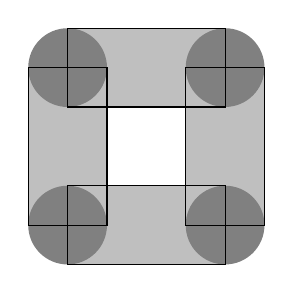
\begin{tikzpicture}
      \fill[lightgray] (0.5,0) rectangle (2.5,1);
      \fill[lightgray] (0.5,2) rectangle (2.5,3);
      \fill[lightgray] (0,0.5) rectangle (1,2.5);
      \fill[lightgray] (2,0.5) rectangle (3,2.5);
      \fill[gray](0.5,0.5) circle (0.5);
      \fill[gray](2.5,0.5) circle (0.5);
      \fill[gray](0.5,2.5) circle (0.5);
      \fill[gray](2.5,2.5) circle (0.5);
      \draw[] (0.5,0) rectangle (2.5,1);
      \draw[] (0.5,2) rectangle (2.5,3);
      \draw[] (0,0.5) rectangle (1,2.5);
      \draw[] (2,0.5) rectangle (3,2.5);
      \end{tikzpicture}}\quad
    \subfloat[]{\label{fig:atc:gps}
      \begin{forest}
        [\name{AosXMonotoneTraits\_2},for tree={concept,edge={-latex}}
          % forked edges
          [\name{AosDirectionalXMonotoneTraits\_2}
            [\name{GeneralPolygonSetTraits\_2}]
          ]
        ]
      \end{forest}}
  \caption{%
    (\subref{fig:csp})~A general polygon with holes bounded by circular arcs and line segments.
    (\subref{fig:atc:gps})~The general point-set cluster.}
  \label{fig:bso2}
\end{figure}

An arrangement data structure is internally used to represent the point set maintained by the general polygon-set; it is possible to obtain it and apply further operations on it, as demonstrated by the following code excerpt.
\framedInputPython[\scriptsize][64]{../../../src/python_scripts/cgalpy_examples/circle_segment_polygons.py}
The bindings for the \iiDArrangementsPackage{} package includes bindings for the geometry traits and the DCEL suitable for Boolean operations. In particular, the traits must model the concept \cppLstinline{GeneralPolygonSetTraits\_2}; see Figure~\ref{fig:atc:gps}.

% -----------------------------------------------------------------------------
\subsection{2D Minkowski Sums}
\label{ssec:modules:ms2}
% -----------------------------------------------------------------------------
Given two sets of points $\calA, \calB \in \Rd$ their Minkowski sum, denoted by $\calA \oplus \calB$, is their point-wise sum, namely the set $\{a+b |\, a \in \calA,b \in \calB\}$. The \cgal{} package \iiDMinkowskiSumsPackage{} contains functions that compute the planar Minkowski sums of two polygons and the planar Minkowski sum of a simple polygon and a disc---an operation also referred to as offsetting or dilating a polygon. The package also supports inner offsetting a polygon (also referred to as insetting), which is equivalent to the complement of the offset of a disk and the complement of a polygon~\cite{cgal:w-rms2-21a}. The \iiDMinkowskiSumsPackage{} module is not associated with any \cmake{} flags (besides the flag \cmakeLstinline{MINKOWSKI_SUM_2_BINDINGS}, which indicates whether to generate bindings for this module). As with the \iiDRegularizedBooleanSetOperationsPackage{} package, the operations supported by this package depends on the \iiDandiiiDGeometryKernelPackage{}, \iiDArrangementsPackage{}, and \iiDPolygonsPackage{} packages. Generating bindings for the \iiDMinkowskiSumsPackage{} module does not require thought enabling the bindings for the \iiDArrangementsPackage{} module (similar to the case of generating bindings of Boolean operations on (linear) polygons supported by the \iiDRegularizedBooleanSetOperationsPackage{} package). The result of the inset and offset operations is a general polygon bounded by line segments and circular arc. Thus, binding for such a type is generated as well.

The function instance \cppLstinline{CGAL::minkowski_sum()} is extremely overloaded. It can be used to compute the Minkowski sum of two polygons either applying the \emph{convex-decomposition} approach or the \emph{reduced-convolution} approach. When applying the \emph{convex-decomposition} approach we first decompose each summand into convex sub-polygons. The function template \cppLstinline{CGAL::minkowski\-_sum_by_full_convolution_2()} applies a third approach, namely \emph{full convolution}. For more information on the various approaches refer to the manual.

There are two overloaded function templates \cppLstinline{CGAL::minkowski_sum()} that apply the \emph{reduced-convolution} approach; both accepts the two polygons as input; one also accepts a specific geometry traits as input (while the other constructs and uses a default one). Each type of the summands must represent either a simple polygon or a polygon with holes. Bellow is the signature of the former, where \cppLstinline{PolygonType1} and \cppLstinline{PolygonType2} can be substituted either with \cppLstinline{Polygon_2} or with \cppLstinline{Polygon_with_holes_2}.
\begin{lstlisting}[style=cppStyle,basicstyle=\scriptsize]
template <typename Kernel, typename Container>
Polygon_with_holes_2<Kernel, Container>
minkowski_sum_2(const PolygonType1<Kernel, Container>& p,
                const PolygonType2<Kernel, Container>& q)
\end{lstlisting}
Thus, given a specific kernel and container types, we get eight overloaded instances that apply the \emph{reduced-convolution} approach in total. (The Container type determines the representation of the polygon extreme points in memory.)

There are two sets of function templates \cppLstinline{CGAL::minkowski_sum()} that apply the \emph{convex-decomposition} approach; all functions accepts the two polygons as input; functions in one set also accept a specific geometry traits as input. As with the functions that apply the \emph{reduced-convolution} approach, each type of the summands must be substituted either with a type that represents a simple polygon or a type that represents a polygon with holes. Each set consists of two function templates; one is parameterized with the type that represents a single decomposition strategy that should be applied to both summands and another one that is parameterized with two types that represents two decomposition strategies that should be applied to the two summands, respectively. The package provides four types of decomposition strategies; however, only two can be applies to polygon width holes. Bellow are the signatures of the two functions that do not accept a traits parameter.
\begin{lstlisting}[style=cppNumberedStyle,basicstyle=\scriptsize,label={lst:msSignatures},caption={Signatures of free functions that compute the 2D Minkwoski sum using the conves-decomposition approach.}]
template <typename Kernel, typename Container,
          typename PolygonConvexDecomposition_2>
Polygon_with_holes_2<Kernel, Container>
minkowski_sum_2(const PolygonType1<Kernel, Container>& p,
                const PolygonType2<Kernel, Container>& q,
                const PolygonConvexDecomposition_2& decomp)

template <typename Kernel, typename Container,
          typename PolygonConvexDecompositionP_2,
          typename PolygonConvexDecompositionQ_2>
Polygon_with_holes_2<Kernel, Container>
minkowski_sum_2(const PolygonType1<Kernel, Container>& p,
                const PolygonType2<Kernel, Container>& q,
                const PolygonConvexDecompositionP_2& decomp_p,
                const PolygonConvexDecompositionQ_2& decomp_q)
\end{lstlisting}
We get 10~overloaded instances of functions that apply the \emph{convex-decomposition} approach, do not accept a traits parameter, and are parameterized with a single decomposition strategy. We get 36~overloaded instances of functions that apply the \emph{convex-decomposition} approach, do not accept a traits parameter, and are parameterized with two decomposition strategies. Thus, given a specific kernel and container types, we get $2 \times (10 + 36) = 92$ overloaded instances of functions that apply the \emph{convex-decomposition} approach.

The \cppLstinline{approximated_inset_2(P, r, eps, oi)} function template accepts a polygon $P$, an inset radius $r$, (a floating-point number\index{number!floating-point}) $\epsilon > 0$, and an output iterator\index{iterator!output} \cppLstinline{oi}, whose value-type must be an instance of the class template \cppLstinline{Gps_circle_segment_traits_2::Polygon_2}. It constructs an approximation of the inset of $P$ by the radius $r$, where the approximation error is bounded by $\epsilon$. The function returns the polygons that approximate the inset polygon through the output iterator \cppLstinline{oi}.

The code excerpt below demonstrates the construction of an approximated inner offset; see
Figure~\ref{fig:ms2:inset}.

\framedInputPython[\scriptsize][35]{../../../src/python_scripts/cgalpy_examples/approx_inset.py}

\begin{SCfigure}[][!htp]
 \begin{tikzpicture}[scale=0.4]
    \coordinate (c1) at (8,3);
    \coordinate (p11) at (8.94868,3.31623);
    \coordinate (p12) at (7.05132,3.31623);
    %
    \coordinate (c2) at (6,7);
    \coordinate (p21) at (6.78087,6.3753);
    \coordinate (p22) at (7,7);      %\draw (6,9) circle (3pt);


    \filldraw [color=polyADarkColor,fill=polyALightColor,thick]
      (4, 0)--(7,0)--(8,3)--(9,0)--(13,0)--(13,8)--(7,8)--(7,9)--
      (13,9)--(13,14)--(0,14)--(0,12)--(6,9)--(6,7)--(2,2)--cycle;
    \filldraw [color=polyCDarkColor,fill=polyCLightColor,thick]
      let \p1 = ($(p11) - (c1)$),
        \p2 = ($(p12) - (c1)$),
        \n0 = {veclen(\x1,\y1)}, % radius
        \n1 = {atan2(\y1,\x1)},  % initial angle
        \n2 = {atan2(\y2,\x2)},   % Final angle
        \p3 = ($(p21) - (c2)$),
        \p4 = ($(p22) - (c2)$),
        \n3 = {veclen(\x3,\y4)}, % radius
        \n4 = {atan2(\y3,\x4)},  % initial angle
        \n5 = {atan2(\y3,\x4)}   % Final angle
      in
        (7,7)--(12,7)--(12,1)--(9.72076,1)--(9.29057,2.29057)--(p11)arc(\n1:\n2:\n0)--
        (6.3932,1.34189)--(6.27924,1)--(4.41421,1)--(3.34,2.07422)--(3.53148,2.31357)--
        (p21)arc(\n4:\n5:\n3)--cycle;
    \filldraw [color=polyCDarkColor,fill=polyCLightColor,thick]
      (1,13)--(12,13)--(12,10)--(7,10)--
      (6.5,9.86603)--
      (6.44721,9.89443)--(4.78885,10.7236)--(1,12.618)--(1,13)--cycle;
      %\draw (7,9) circle (3pt);
      %\draw (6,9) circle (3pt);
  \end{tikzpicture}
    %\caption{%
  \caption{%
      The inset (yellow) of a polygon (blue) with a tight corridor consists of two general polygons bounded by line segments and circular arcs.}
  \label{fig:ms2:inset}
\end{SCfigure}
